%===================================== CHAP 4 =================================

\chapter{Research Design and Methodology}
Over the course of this project, both quantitative and qualitative data gathering methods and analysis were employed. Both of the methods offered something valuable to the project, and using both allowed us to gather the data best suited for the thesis. In the early stages quantitative data, such as surveys, were used to gather opinions and thoughts from potential users of the program. Using these surveys, we could create a base to build from, and develop a better prototype. With this prototype finished, more qualitative measures were used to gather more specific and more detailed data. Figure \ref{fig:researchMethod} provided an overview of the research process applied in this thesis, from the strategy, data generation methods and data analysis methods.  

\begin{figure}[!ht]
     \centering
     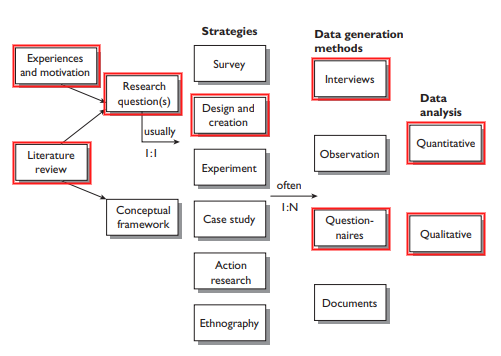
\includegraphics[width=.8\textwidth]{./fig/researchMethodology/OatesResearch.png}
     \captionsetup{width=0.8\linewidth}
     \caption{Model of the research process adapted from Oates \cite{oates2005researching}. The red outlined boxes are methods used in this thesis.}
     \label{fig:researchMethod}
 \end{figure}

\section{Design and Creation Research}
\label{sec:designCreationResearch}
One of the more common research methodologies in computer science, Design and Creation Research uses common development techniques and adapts them for research and is also the research methodology that will be used for this thesis. It focuses on development of new IT products, also called artefacts \cite{oates2005researching}. In the case of this paper, the artefact being developed is a prototype aiming to figure out whether or not collaboration is conducive to workplace training in virtual reality. This type of research can be split into a few different types, mostly depending on whether the artefact itself is the end goal, a vehicle for research or if the focus is on the development process itself. The most relevant case for this project is the second case. To expand upon this one slightly, to say that the artefact is a vehicle for the research means that while the artefact itself is important, its \textit{usage} in real life is what's really important. By developing something that can be used in real life, it is possible to point to something concrete and measure the perceived effects the artefact has on the system it is introduced to.

While the artefact in this project is a vehicle for the research, the aim is to have one of the pre-existing workplace training applications working with collaborative elements at close to 100\% functionality, so that others may continue developing the application later with relative ease. The most important part is still to see whether or not the end product can heighten the efficacy of the VR workplace training project.


\section{Development methodology}
The primary type of development used in the project can best be described as a variant of agile software development. Agile development refers to certain principles that were written down in the 2001 article \textit{Manifesto for Agile Software Development}\cite{beck2001manifesto}. This manifesto decries the old method of rigid development that was very resistant to change. Over the course of this project, feedback is sought at every level, hoping to improve the software both for the customer and the users, and that means that it must be open to change when it needs to.

There will be multiple iterations and phases of the project, each building upon the last. Three major phases were roughly planned out at the beginning of the project, with each containing multiple iterations as priorities shift based on feedback. These three phases are discussed in more detail in chapters \ref{chap:phase1}, \ref{chap:phase2} and \ref{chap:phase3}, respectively.


\section{Methods to Answer Research Questions}


\section{User testing}
User tests are an important part of agile development. They are one of the primary means of gathering relevant feedback from the people who will actually be using your product. A lot of care goes into creating the tests and making sure that the data extracted from them is sound and valid. The tests needs to specific enough to showcase or test the aspect you are focusing on, but not so specific that it becomes an unnatural situation that does not represent the actual product.

\textcolor{red}{SKRIV LITT MER I DYDBE OM USER TESTS, HVA ER DE ETC}

Most of the tests performed with the target audience has been done in collaboration with NAV. With their help, testers in the target group were gathered, and they could then try out the application collaboratively. The experience would be supervised by us, ready to guide or help if they struggled with the basic VR interactions, as the testers had quite varying levels of familiarity with VR. Once they had finished the tasks that were available to them they were asked questions through a semi-structured interview that had been planned out in advance.


\subsection{The Surveys}
In the beginning phases of the project, it was deemed important to get an overview of the general attitude of the target audience when it came to VR. As such, plans were made to conduct surveys of different parts of the target audience. This included both young job seekers, as well as NAV employees. For the first group, the most significant knowledge to be gained was what young job seekers felt was helpful and what was not when it came to VR. The previously developed application at the IMTEL lab suited that purpose excellently, and could be used to convey the possibilities, as well as the limitations of VR, and hopefully evoke useful feedback.

For the second group, NAV employees, it was important to figure out how they usually worked with the job seekers. What did their workflow look like before, and how could the artefact of this project fit into that?


\subsection{Expert tests}
Since most of the work of this project was done at the IMTEL lab, opportunities presented themselves for us to gather feedback and advice. Throughout the year, people from multiple fields and disciplines stopped by the lab for various reasons, and most were quite open to some discussion about the project. The multidisciplinary nature of the project meant that even if they were not necessarily well versed in every aspect, they still had some valuable input for us to consider.

As such, during the course of the project we often got to test the current iteration on people from different people. These tests may have been more informal than the standard user tests that were performed, but they offered a lot of insight that we may not have considered on our own. In the later sections concrete examples of these discussions will be provided, and the information gathered from them. 




\cleardoublepage